\chapter{Resultados y evaluación}
\label{chap:resultados-evaluacion}

Este capítulo presenta los avances que pueden reconstruirse a partir de los resultados guardados. Los resultados principales corresponden a Llama-3.3-70B V3 y al registro de Mistral-7B V3. Se distingue la estimación dentro de muestra de la evaluación fuera de muestra, y los resultados diagnósticos de los ensayos conductuales exploratorios. La discusión y los límites se desarrollan en el Capítulo~\ref{chap:discusion}.

\section{Resultados, análisis e interpretación}
\label{sec:resultados}
\subsection{Alcance de las ejecuciones}

El corpus ampliado está construido y validado con 96 pares, pero las ejecuciones disponibles emplean 42 pares. En cada una, esos pares producen 168 entradas en las cuatro condiciones; para una sonda de un formato hay 84 observaciones dañinas y benignas. Las variantes no incrementan el número de unidades independientes. La Tabla~\ref{tab:corridas} identifica el soporte de cada ejecución.
\begin{table}[htbp]\centering\small
\begin{adjustbox}{max width=\textwidth}
\begin{tabular}{@{}lrrrl@{}}\toprule
Modelo & Pares & Capas & Referencia & Soporte \\\midrule
Llama-3.3-70B V3 & 42 & 20 de 80 & 76 & JSON y activaciones \\
Mistral-7B V3 & 42 & 16 de 32 & 30 & Registro de ejecución \\
Qwen3-8B (previo) & 42 & 18 de 36 & 32 & JSON histórico \\
Qwen3-32B (previo) & 42 & 32 de 64 & 46 & JSON histórico \\
\bottomrule\end{tabular}\end{adjustbox}
\caption{Ejecuciones disponibles. Qwen se conserva como evidencia exploratoria; no se trata como réplica del pipeline corregido. El paquete causal de Mistral no está completo localmente.}\label{tab:corridas}\end{table}

La capa de referencia maximiza el desplazamiento en el barrido completo y se usa para describir magnitudes. La inferencia separada de selección de capa se reporta más adelante. Los valores de Mistral proceden de tablas impresas y conservan su precisión redondeada; no se reconstruye un JSON ausente ni se añaden decimales inferidos.

\subsection{Línea base y capacidad discriminativa}

La dirección conversacional se estima en cuatro de cinco folds de pares y se evalúa en el restante. La Tabla~\ref{tab:linea_base} reporta los AUROC de sus puntajes retenidos. Mide discriminación entre etiquetas de contenido, no rechazo efectivo del modelo.
\begin{table}[htbp]\centering\small
\begin{adjustbox}{max width=\textwidth}
\begin{tabular}{@{}lrrrr@{}}\toprule
Modelo & Capa & AUROC chat & AUROC agente & Diferencia \\\midrule
Llama V3 & 76 & 0{,}9779 & 0{,}9195 & 0{,}0584 \\
Mistral V3 & 30 & 0{,}9478 & 0{,}7851 & 0{,}1627 \\
\bottomrule\end{tabular}\end{adjustbox}
\caption{AUROC de la dirección conversacional fuera de muestra, con cinco folds por pares y 42 pares por modelo. Cada comparación de formato utiliza la misma dirección de entrenamiento.}\label{tab:linea_base}\end{table}

En Llama el IC de remuestreo de la diferencia de AUROC es $[0{,}0113;\ 0{,}1128]$; el de chat es $[0{,}9490;\ 0{,}9955]$ y el de agente $[0{,}8560;\ 0{,}9734]$. Son intervalos condicionales a los puntajes cross-fit guardados. Para Mistral no se dispone localmente del conjunto de puntajes ni de un intervalo equivalente exportado. La pérdida puntual es mayor en Mistral, pero no se realiza una prueba formal entre modelos ni se atribuye la diferencia exclusivamente a su tamaño.

La sonda logística conversacional es otra medida. En Llama, capa 76, su AUROC medio en diez repeticiones de cinco folds es $0{,}9677$, con desviación entre folds $0{,}0373$ e IC corregido Nadeau--Bengio $[0{,}9285;\ 1]$; el control permutado es $0{,}5152$. La desviación entre folds no es un intervalo de confianza. La muestra completa produce AUROC de entrenamiento $1$, que no se usa como evidencia de generalización. La curva de la dirección y la curva de una sonda no deben confundirse, ni la cercanía de dos sondas demuestra equivalencia.
\begin{figure}[htbp]\centering
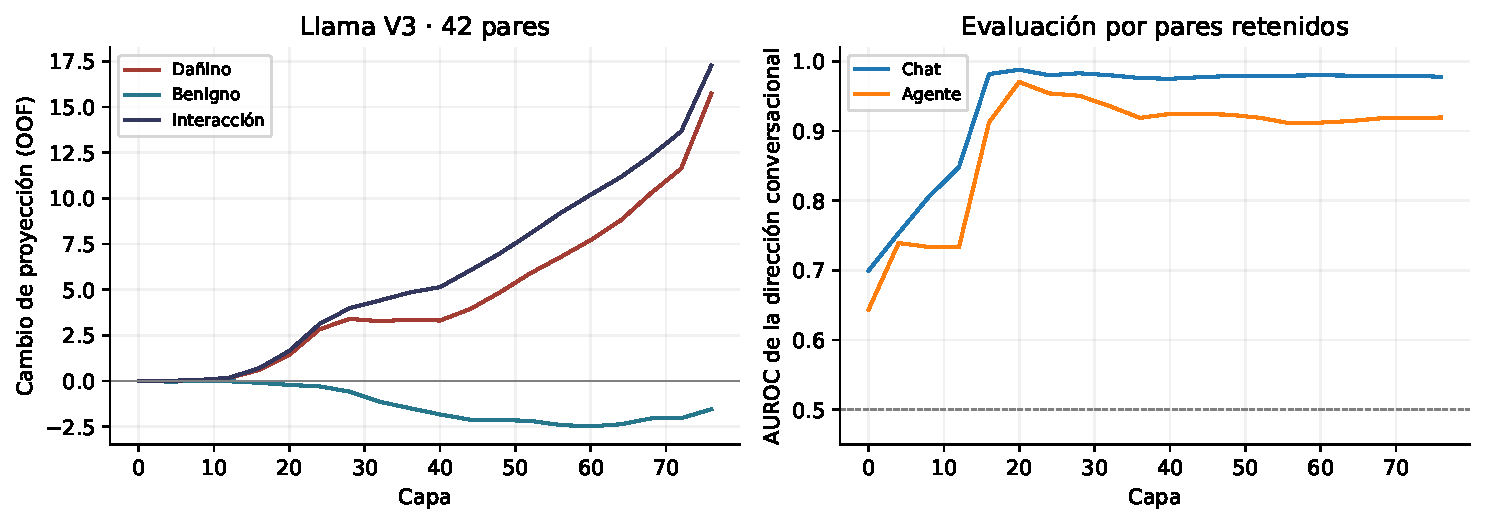
\includegraphics[width=0.94\textwidth]{avance_llama_capas}
\caption{Llama V3 sobre 42 pares. Izquierda: desplazamientos e interacción con direcciones cross-fit. Derecha: AUROC fuera de muestra de la dirección conversacional. Cada capa es una medición correlacionada del mismo corpus.}\label{fig:auroc_capa}\end{figure}

\subsection{Desplazamiento y control benigno}
\label{sec:desplazamiento}

El resultado central se expresa mediante cambios intra-par. Una proyección menor no demuestra por sí sola menor rechazo: es una medida geométrica. El brazo benigno permite descartar un desplazamiento idéntico de ambas clases sobre el eje, pero no identifica por sí solo el mecanismo completo ni elimina toda posible interacción de longitud y contenido.
\begin{table}[htbp]\centering\small
\begin{adjustbox}{max width=\textwidth}
\begin{tabular}{@{}lrrrr@{}}\toprule
Modelo & $\Delta p_h$ & $\Delta p_b$ & $\Delta^2p$ & IC 95\,\% interacción \\\midrule
Llama V3 & 15{,}7244 & -1{,}5438 & 17{,}2682 & $[14{,}9074;\ 19{,}4547]$ \\
Mistral V3 & 7{,}8359 & -0{,}5818 & 8{,}4178 & $[7{,}0992;\ 9{,}6758]$ \\
\bottomrule\end{tabular}\end{adjustbox}
\caption{Desplazamiento fuera de muestra, con dirección reajustada por fold. La interacción respeta el pareado dañino--benigno. Las unidades crudas no se comparan entre modelos.}\label{tab:gap}\end{table}

Las interacciones retenidas son positivas y sus intervalos excluyen cero. El test intra-par guardado reporta $p\simeq 10^{-4}$ en ambos casos, a la resolución de 10.000 permutaciones. La fracción común es aproximadamente $-9{,}8\,\%$ en Llama y $-7{,}4\,\%$ en Mistral. En ambos, el cambio benigno es pequeño frente al dañino y su contraste individual no permite afirmar un movimiento benigno distinto de cero al nivel $0{,}05$. La evidencia se concentra en el contraste entre brazos, no en declarar ausencia exacta de efecto en el benigno.

\subsection{Escala del efecto}
\label{sec:escala}

La separación cruda mezcla capacidad discriminativa y escala de proyección. En Llama, fuera de muestra, su pérdida es $82{,}6\,\%$, mientras la separación estandarizada cae $43{,}7\,\%$ y el AUROC pierde $0{,}0584$. En Mistral las pérdidas impresas son $84{,}7\,\%$, $63{,}8\,\%$ y $0{,}1627$, respectivamente. Ninguna cifra cruda debe presentarse como porcentaje de pérdida de seguridad.
\begin{table}[htbp]\centering\small
\begin{adjustbox}{max width=\textwidth}
\begin{tabular}{@{}lrrrr@{}}\toprule
Modelo & $d_{\rm chat}$ & $d_{\rm ag}$ & Pérdida en $d$ & $\kappa$ \\\midrule
Llama V3 & 3{,}2051 & 1{,}8036 & 43{,}7\,\% & 0{,}309 \\
Mistral V3 & 2{,}5289 & 0{,}9163 & 63{,}8\,\% & 0{,}422 \\
\bottomrule\end{tabular}\end{adjustbox}
\caption{Separación entre clases en unidades estandarizadas, obtenida sobre puntajes fuera de muestra. Estos valores de $d$ difieren del tamaño pareado del cambio de formato.}\label{tab:escala}\end{table}

\subsection{Comportamiento por explicitud}
\label{sec:estratos}

El análisis disponible utiliza los estratos originales de 18, 14 y 10 pares. El corpus ampliado cuenta con 42, 24 y 30, pero esos tamaños no se transfieren a las estimaciones siguientes.
\begin{table}[htbp]\centering\small
\begin{adjustbox}{max width=\textwidth}
\begin{tabular}{@{}llrrrr@{}}\toprule
Modelo & Estrato & Pares & Chat & Agente & Pérdida \\\midrule
Llama V3 & Explícito & 18 & 0{,}9907 & 0{,}9290 & 0{,}0617 \\
Llama V3 & Contextual & 14 & 0{,}9847 & 0{,}9643 & 0{,}0204 \\
Llama V3 & Apariencia legítima & 10 & 0{,}9400 & 0{,}8900 & 0{,}0500 \\
Mistral V3 & Explícito & 18 & 0{,}9722 & 0{,}8827 & 0{,}0895 \\
Mistral V3 & Contextual & 14 & 0{,}9439 & 0{,}7398 & 0{,}2041 \\
Mistral V3 & Apariencia legítima & 10 & 0{,}9000 & 0{,}7100 & 0{,}1900 \\
\bottomrule\end{tabular}\end{adjustbox}
\caption{AUROC por explicitud sobre puntajes fuera de muestra. El pequeño tamaño de los estratos y la ausencia de intervalos por estrato impiden establecer una ordenación poblacional firme.}\label{tab:estratos}\end{table}

La pérdida puntual máxima de Llama aparece en el estrato explícito y la de Mistral en el contextual. Por tanto, no hay una jerarquía universal de degradación según explicitud en estas ejecuciones. El estrato de apariencia legítima conserva señal por encima del azar en ambos modelos, pero no se interpreta como garantía de detección de solicitudes encubiertas nuevas.
\begin{figure}[htbp]\centering
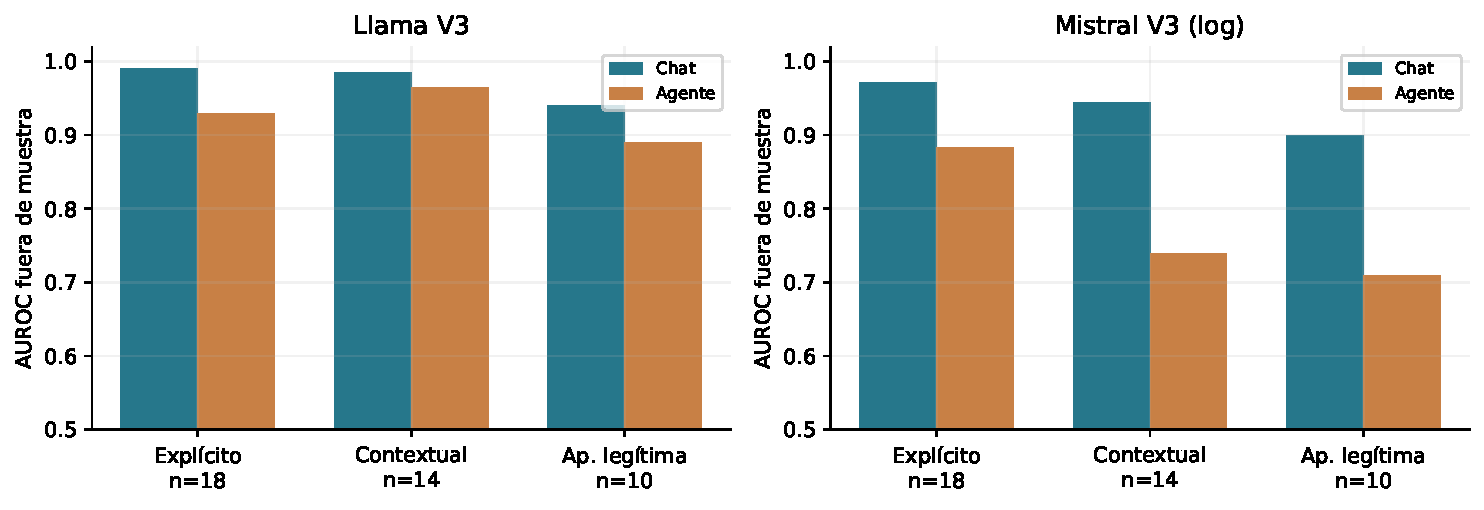
\includegraphics[width=0.94\textwidth]{avance_estratos}
\caption{Discriminación por explicitud en las dos ejecuciones principales. Ambas usan 42 pares; las barras son estimaciones puntuales, no diferencias estadísticamente contrastadas entre modelos.}\label{fig:cmp_estratos}\end{figure}

\subsection{Reorientación y monitores por estimador}
\label{sec:rotacion}

En Llama, capa 76, el coseno de muestra completa entre direcciones de medias es $0{,}2128$. Las fiabilidades entre mitades disjuntas son $0{,}9010$ en chat y $0{,}9220$ en agente. La estimación normalizada por el techo de fiabilidad da coseno $0{,}2204$ y ángulo descriptivo de unos $77^\circ$. La alineación es baja, pero no corresponde al coseno $0{,}051$ que la versión anterior atribuía a ese modelo.

La comparación logística produce coseno de muestra completa $0{,}0744$ y fiabilidades mucho menores, $0{,}2522$ y $0{,}2832$. Esa menor reproducibilidad obliga a interpretar con más cautela el ángulo. Las dos medidas no se promedian ni se sustituyen una por otra.
\begin{figure}[htbp]\centering
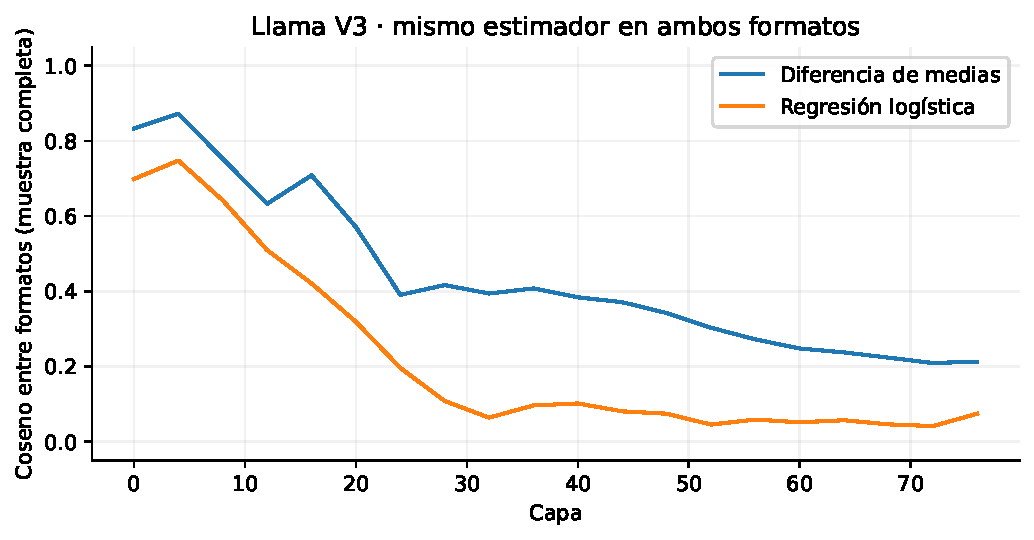
\includegraphics[width=0.94\textwidth]{avance_rotacion}
\caption{Llama V3: cosenos de muestra completa entre formatos, usando el mismo estimador en ambos. Los valores no son una prueba causal y deben leerse junto con la fiabilidad descrita en el texto.}\label{fig:cmp_rotacion}\end{figure}
\begin{table}[htbp]\centering\small
\begin{adjustbox}{max width=\textwidth}
\begin{tabular}{@{}lrrr@{}}\toprule
Modelo / estimador & AUROC OOF & $F_1$ OOF & FPR OOF \\\midrule
Llama / medias & 0{,}9707 & 0{,}8434 & 0{,}1429 \\
Llama / logística & 0{,}9926 & 0{,}9367 & 0{,}0000 \\
Mistral / logística (log) & 0{,}9347 & 0{,}8250 & 0{,}1190 \\
\bottomrule\end{tabular}\end{adjustbox}
\caption{Monitores agénticos evaluados por cinco folds. En Llama se usa capa 76; en Mistral, capa 30. El AUROC corresponde a la media de folds y $F_1$ al protocolo de umbrales retenidos; las métricas no son intercambiables.}\label{tab:monitores}\end{table}

El cero de falsos positivos de la logística de Llama corresponde a 42 benignos de este corpus. No demuestra una tasa poblacional nula ni seguridad de despliegue. La señal agéntica es aprovechable por un monitor ajustado en ese formato; eso no demuestra que el mecanismo interno de rechazo use espontáneamente el mismo eje.

\section{Evaluación y validación}
\label{sec:evaluacion-resultados}
\subsection{PCA del contraste conversacional}

PCA se ajusta sobre activaciones conversacionales concatenadas y centradas globalmente, según el procedimiento de métodos. La Tabla~\ref{tab:pca} incorpora los resultados que faltaban en la versión anterior. Los de Llama se comprobaron además desde las activaciones guardadas mediante el autovector principal de la matriz de Gram.
\begin{table}[htbp]\centering\small
\begin{adjustbox}{max width=\textwidth}
\begin{tabular}{@{}lrrr@{}}\toprule
Modelo & Capa & $|\cos(\mathrm{PC1},\hat{\bm{r}})|$ & Varianza de PC1 \\\midrule
Llama V3 & 28 & 0{,}9934 & 36{,}53\,\% \\
Llama V3 & 56 & 0{,}9936 & 25{,}91\,\% \\
Llama V3 & 76 & 0{,}9894 & 20{,}13\,\% \\
Mistral V3 & 18 & 0{,}968 & 30{,}3\,\% \\
Mistral V3 & 30 & 0{,}952 & 28{,}7\,\% \\
\bottomrule\end{tabular}\end{adjustbox}
\caption{Validación geométrica descriptiva, dentro de muestra. La alineación con PC1 no sustituye la evaluación fuera de muestra del AUROC.}\label{tab:pca}\end{table}
\begin{figure}[htbp]\centering
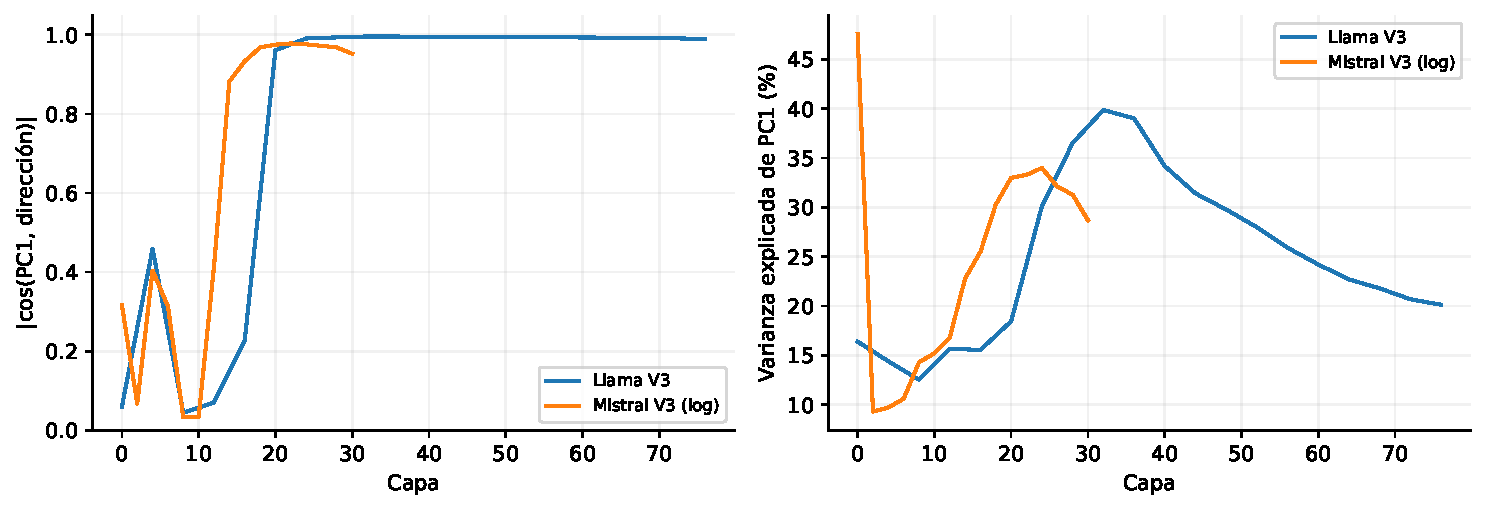
\includegraphics[width=0.94\textwidth]{avance_pca}
\caption{Alineación de PC1 y proporción de varianza explicada a lo largo de las capas. Las posiciones de capa son propias de cada arquitectura y los puntos de Mistral conservan la precisión impresa del log.}\label{fig:pca}\end{figure}

En capas iniciales el contraste no siempre coincide con PC1. En las capas profundas mostradas sí presenta alineación elevada, sin que PC1 explique toda la varianza: por ejemplo, en la capa 76 de Llama explica $20{,}13\,\%$. Este resultado respalda una estructura geométrica dominante de la muestra en esas capas, no la identidad entre un componente principal y una causa del rechazo.

\subsection{Circularidad y selección de capa}

En Llama, capa 76, el desplazamiento ingenuo es $16{,}2776$ y el cross-fit es $15{,}7244$: la diferencia equivale al $3{,}5\,\%$ del valor corregido. En Mistral, capa 30, pasa de $8{,}0227$ a $7{,}8359$, un $2{,}4\,\%$. La corrección reduce el efecto y este conserva su signo. Los conteos cross-fit son 42/42 y 39/42 decrecientes, respectivamente; constituyen una comprobación descriptiva sobre el corpus completo.

Para evitar reutilizar los pares que seleccionan una capa, la inferencia separada utiliza solo la otra mitad. La Tabla~\ref{tab:seleccion} resuelve la ambigüedad del conteo antiguo de 39/42: no debe presentarse como un conteo exclusivo de inferencia.
\begin{table}[htbp]\centering\small
\begin{adjustbox}{max width=\textwidth}
\begin{tabular}{@{}lrrrrr@{}}\toprule
Modelo & Selección & Inferencia & Capa & Decrecen & $\Delta p$ inferencia \\\midrule
Llama V3 & 21 & 21 & 76 & 21/21 & 16{,}5899 \\
Mistral V3 & 21 & 21 & 30 & 19/21 & 7{,}6873 \\
\bottomrule\end{tabular}\end{adjustbox}
\caption{Selección e inferencia sobre mitades disjuntas de pares. Los 42/42 o 39/42 del cross-fitting global no son el denominador de esta prueba.}\label{tab:seleccion}\end{table}

El intervalo de inferencia de Llama es $[14{,}0276;\ 18{,}9079]$ y el de Mistral $[6{,}0074;\ 9{,}1634]$. Sus pruebas de signos arrojan aproximadamente $9{,}54\times10^{-7}$ y $2{,}21\times10^{-4}$; ambas quedan bajo los umbrales Bonferroni $0{,}0025$ y $0{,}003125$. Sobre 200 particiones aleatorias, cada ejecución selecciona su misma capa en el $100\,\%$ de los casos guardados. Estas particiones describen estabilidad sobre el corpus observado; no multiplican el tamaño de muestra.

La prueba de signos depende de la dirección utilizada. Su invariancia se limita a reescalados positivos, no a cambios del eje. La separación entre ajuste y evaluación protege frente a circularidad, sin eliminar todos los supuestos de muestreo.

\section{Ensayos conductuales e intervención exploratoria}
\label{sec:conductual}

Llama V3 conserva las generaciones y sus etiquetas heurísticas. En solicitudes dañinas, el rechazo sin intervención pasa de 38/42 en chat ($90{,}5\,\%$) a 23/42 en agente ($54{,}8\,\%$). Dieciséis pares dejan de rechazar y uno cambia en sentido contrario, con McNemar exacto $p=0{,}000275$. En benignos las tasas son 5/42 y 1/42. Estas etiquetas describen respuestas generadas, no ejecución de tareas mediante herramientas, y su auditoría humana está pendiente.

Como ejemplo de intervención se reporta la capa 56, declarada explícitamente en la configuración de ese ensayo; es distinta de la capa 76 usada para el diagnóstico principal. Se evalúan 19 dañinos y 41 benignos que inicialmente no eran rechazados en formato agéntico.
\begin{table}[htbp]\centering\small
\begin{adjustbox}{max width=\textwidth}
\begin{tabular}{@{}lrrr@{}}\toprule
Dosis & Rechazo dañino & Control aleatorio & Rechazo benigno \\\midrule
0{,}5 & 6/19 & 1/19 & 0/41 \\
1{,}0 & 12/19 & 1/19 & 5/41 \\
2{,}0 & 19/19 & 1/19 & 40/41 \\
4{,}0 & 19/19 & 1/19 & 33/41 \\
\bottomrule\end{tabular}\end{adjustbox}
\caption{Llama V3, intervención exploratoria en capa 56. El control aleatorio tiene igual norma. Los denominadores corresponden a subconjuntos que no rechazaban inicialmente; no son los 42 pares completos.}\label{tab:causal}\end{table}
\begin{figure}[htbp]\centering
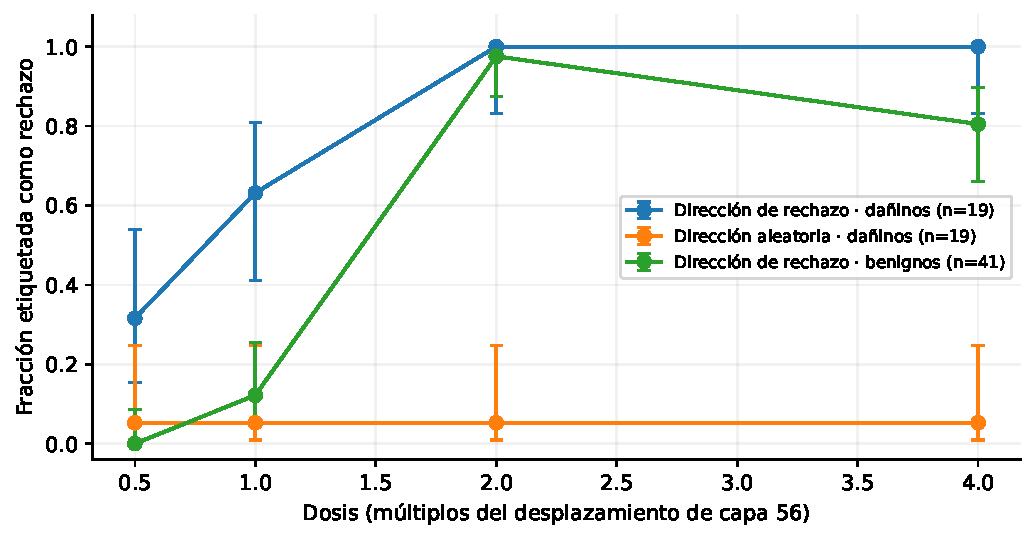
\includegraphics[width=0.94\textwidth]{avance_intervencion}
\caption{Respuesta a la dosis en capa 56. Barras: intervalos binomiales guardados. Una dosis que induce rechazo también en benignos no constituye una reparación selectiva.}\label{fig:causal}\end{figure}

En dosis 1 el rechazo dañino es 12/19 con dirección de rechazo y 1/19 con control aleatorio; McNemar pareado $p=0{,}000977$. El brazo benigno rechaza 5/41. En dosis 2 el rechazo dañino alcanza 19/19, pero también 40/41 benignos. El ensayo apoya un efecto de la adición sobre la conducta etiquetada en estas condiciones y muestra un costo de sobrerrechazo. No demuestra que la reorientación observada explique por sí sola el fallo ni resuelve la calibración de una defensa. Los valores $p$ por dosis son exploratorios y no están corregidos por todos los contrastes de capas y dosis.

Mistral conserva una línea base impresa de 19/42 rechazos dañinos en chat y 5/42 en agente, con McNemar $p\simeq0{,}0013$. Su registro termina durante la intervención; por ello no se presenta una curva causal completa ni se infiere su desenlace.

\section{Evidencia exploratoria de Qwen}

Los JSON históricos de Qwen usan igualmente 42 pares. En Qwen3-8B, capa 32, el AUROC held-out de la dirección conversacional es $0{,}5176$ en chat y $0{,}5108$ en agente: esta ejecución no establece una línea base discriminativa suficiente en esa capa. En Qwen3-32B, capa 46, los valores son $0{,}9694$ y $0{,}9558$. La configuración exportada es menos completa y no acredita todos los controles actuales. Se conservan como antecedentes experimentales, sin utilizarlos para sostener una réplica uniforme entre familias ni una ley de escala. Repetirlos con la versión corregida y el corpus ampliado es parte del trabajo pendiente.
